%%%%%%%%%%%%%%%%%%%%%%%%%%%%%%%%%%%%%%%%%%%%%%%%%%%%%%%%%%%%%%%%%%%%%%%%
\chapter{Grundlagen und Hintergründe}
\label{sec:fundamentals}
%%%%%%%%%%%%%%%%%%%%%%%%%%%%%%%%%%%%%%%%%%%%%%%%%%%%%%%%%%%%%%%%%%%%%%%%

Dieses Kapitel beschreibt Grundlagen und Konzepte, die eine wichtige Rolle als Fundament für das Verständnis der Arbeit einnehmen. In erster Linie wird die Kommunikationstechnologie Near Field Communication (NFC) und ihre Funktionsweise vorgestellt. Es soll behandelt werden, wie NFC technisch umgesetzt ist und mithilfe welcher Komponenten und Methoden die drahtlose Kommunikation erfolgt. Außerdem soll auf die Ausführung der Technologie auf mobilen Android Geräten eingegangen und Sicherheitsrisiken und -konzepte beschrieben werden. Ein äußerst relevanter Punkt im Zusammenhang mit dieser Arbeit ist die Relay Attacke. Das Prinzip hinter diesem Angriff und dessen praktische Ausführung werden ebenfalls behandelt. 

\section{Near Field Communication (NFC)}

Near Field Communication ist eine drahtlose Datenübertragungstechnologie ähnlich wie Bluetooth oder WLAN, mit der auf einfachem und schnellem Weg kleinere Datenmengen 
über kurze Distanzen übertragen werden können. Im Vergleich zu anderen kontaktlosen Übertragungsmöglichkeiten muss bei NFC allerdings keine Kopplung der Geräte, die an der Datenübertragung teilnehmen wollen, stattfinden. Befindet sich ein NFC-kompatibles Gerät in der Nähe eines anderen, wird das Senden und Empfangen von Informationen automatisch
gestartet, was die Benützung der Technologie sehr angenehm und einfach gestaltet. 

Erstmals wurde die Entwicklung von NFC im Jahr 2002 von Philips und Sony bekanntgegeben \cite{sonyPhillipsNfcPressRelease}, die zwei Jahre darauf gemeinsam mit Nokia das NFC Forum, einen Non-Profit Industrieverband zur Entwicklung der Technologie und deren Spezifikation, gründeten \cite{nfcHistory, nfcForum}. Die Organization hat bis zum Jahr 2018 insgesamt 16 Spezifikationen der NFC Technologie veröffentlicht und zählt zahlreiche einflussreiche Unternehmen wie Apple, Google, Intel, Sony, Visa, Mastercard und viele weitere zu seinen Mitgliedern \cite{nfcForum}. 

Zusätzlich zu den Spezifikationen des NFC Forums ist NFC durch den ISO 18092 Standard sowie ETSI TS 102 190 Standard standardisiert, der die Kommunikationsmodi für das NFC Interface und das NFC Protokoll beschreibt \cite{iso:iec18092:2013, etsi:ts:102:190}.

\subsection{Die Funktionsweise von NFC}

Die Basis für die Funktionsweise von NFC bildet das Prinzip der magnetischen Induktion \cite{introToRfid}. Dieses allgemein bekannte Prinzip besagt, dass ein sich ändernder elektrischer Strom ein Magnetfeld hervorruft und umgekehrt ein sich änderndes Magnetfeld, elektrischen Strom in einem Leiter erzeugt. Ein NFC Chip besteht daher grundlegend aus einer Spule, die mit elektrischem Strom versorgt werden kann und dadurch ein elektromagnetisches Feld hervorruft. Dieses besitzt eine festgelegte Frequenz im 13,56 MHz Bereich \cite{introToRfid} und kann in der nahen Umgebung des Erzeugers genutzt werden, um einen Kommunikationskanal aufzubauen. NFC-fähige Geräte können grundsätzlich in zwei Modi operieren: aktiv und passiv. 
\newline

\textbf{Passiver Modus}

Im passiven Modus nehmen an der Kommunikation sowohl ein aktiver als auch ein passiver Partner teil. 
Der aktive Teilnehmer versorgt den NFC Chip des Gerätes mit elektrischem Strom wodurch ein elektromagnetisches Feld erzeugt wird. Wird ein passiver NFC Chip ohne eigene Stromversorgung, auch Tag genannt, in die Nähe des aussendenden Gerätes gebracht, verursacht dies in der Spule des passiven Chips wiederum einen elektrischen Strom, der für den Betrieb genutzt werden kann. 
Mithilfe dieser Methode können Daten übertragen werden indem der aktive Erzeuger sein Feld direkt verändert. Diese Änderungen können als Daten wahrgenommen und gesendet werden. Der passive Kommunikationspartner modifiziert das Feld durch das Entziehen von Energie, wodurch Feldschwankungen, die vom Feldverursacher als Informationen identifiziert werden können, entstehen \cite{Madlmayr2014}. 
\newline

\textbf{Aktiver Modus}

Im aktiven Modus generiert und verändert jeder der Kommunikationspartner sein eigenes elektromagnetisches Feld, was vom jeweils anderen Teilnehmer als Information interpretiert werden kann \cite{Madlmayr2014}. 
\newline

Geräte, die NFC unterstützen, sind typischerweise in der Lage zwischen aktivem und passivem Modus zu wechseln und befinden sich standardmäßig im passiven Zustand \cite{cuno:nfc}. Vor der Initiierung einer Verbindung über NFC wird jedem Kommunikationsteilnehmer eine aktive bzw. passive Rolle zugeteilt \cite{Madlmayr2014}. 

Neben den Modi, in welchen ein Gerät, das zur Datenübertragung mittels NFC fähig ist, sich befinden kann, unterscheidet man bei der Kommunikation über die drahtlose Technologie zwischen den drei Modi Peer-to-Peer, Read/Write und Card Emulation, die nachfolgend genauer beleuchtet werden. Um eine Datenübertragung über diese Modi zu ermöglichen, besitzt ein NFC-fähiges Gerät einen Host Controller, ein Secure Element (SE) sowie den NFC Chip. Der Chip sorgt für die Umwandlung der digitalen Signale in die analogen Feldveränderungen und umgekehrt. Das Secure Element ist eine sichere und modifikationsgeschützte Umgebung zur Ausführung von Code und beinhaltet typischerweise mehrere Applikationen, die gestartet werden können. Die Implementierung des SE kann auch vollständig softwarebasiert erfolgen und im Regelfall ist es dazu in der Lage, echte Smartcards zu emulieren. 
Der Host Controller ist verantwortlich für die Steuerung des NFC Chips sowie für die Kommunikation mit dem Secure Element \cite{Madlmayr2014}. Diese Komponente sorgt demnach dafür, dass die Signale des elektromagnetischen Feldes, die vom NFC Chip empfangen werden, nach deren Umwandlung an das SE weitergeleitet werden, um dort bestimmte Anweisungen auszuführen. 
\newline
\newline
Die Kommunikation über NFC kann in einem der folgenden drei Modi durchgeführt werden: 
\newline
\newline
\textbf{Peer-to-Peer Modus}

Befinden sich zwei Geräte im Peer-to-Peer Modus, können Daten über eine bidirektionale Verbindung in beiden Richtungen untereinander ausgetauscht werden. Diese Daten können Nachrichten, Kontakte, Bilder oder jegliche andere Art von Informationen beinhalten. Beim Senden der Nachrichten befindet sich der Sender im aktiven Modus und erzeugt somit sein eigenes elektromagnetisches Feld. Der Empfänger der Nachrichten befindet sich beim Empfangen der Informationen im passiven Modus \cite{Madlmayr2014, nfcHealthMonitoring}. 
\newline
\newline
\textbf{Read/Write Modus}

Ein NFC Gerät, dass sich im Read/Write Modus befindet, ist in der Lage, Informationen von passiven NFC Tags, die keine eigene Energieversorgung besitzen, zu lesen, sowie Daten auf ihnen zu speichern bzw. zu modifizieren. Auf den Tags können sich unterschiedlichste Informationen wie Weblinks oder WLAN Verbindungsinformationen befinden. Je nach Art der gespeicherten Information führt das NFC Gerät diverse Aktionen, wie beispielsweise ein Video im Webbrowser zu öffnen oder Treuepunkte auf einer Kundenkarte zu verändern, aus \cite{Madlmayr2014, nfcHealthMonitoring}. 
\newline
\newline
\textbf{Card Emulation Modus}

Der Card Emulation Modus dient dazu, eine kontaktlose Smartcard zu emulieren. Smartcards verfügen über keine eigene Energieversorgung weshalb sich das sie emulierende NFC Gerät im passiven Modus befindet. Card Emuation ist das Gegenteil des Read/Write Modus, da hier das NFC Gerät die exakt umgekehrte Rolle bei der Datenübertragung einnimmt. Mithilfe dieser Datenübertragungsmethode kann eine kontaktlose Zahlung mit dem NFC Gerät anstelle einer echten Karte durchgeführt werden. Durch die Virtualisierung der Smartcard wird darüber hinaus die Möglichkeit geboten, vielfache unterschiedliche Karten auf demselben Gerät zu simulieren und Zahlungen damit durchzuführen \cite{Madlmayr2014}. 

\subsection{Zahlungen mittels NFC}

Um kontaktlose Zahlungen über NFC durchzuführen, werden in erster Linie eine Smartcard sowie ein Smartcard-Reader benötigt, die das NFC Protokoll unterstützen. Nachfolgend sollen diese Komponenten sowie der Ablauf einer kontaklosen Zahlung über die NFC Technologie genauer erläutert werden. 

\subsubsection{Smartcards}

  Unter einer Smartcard, die auch als Integrated Circuit Card (ICC) bzw. Chipkarte bezeichnet wird, versteht man in erster Linie eine Plastikkarte, die einen integrierten Schaltkreis besitzt. Dieser kann sowohl zur Speicherung von Dateien sowie zur Verarbeitung von Instruktionen und zur Ausführung von Programmen verwendet werden \cite{lexikonSmartcard}. Beispiele für Smartcards sind handelsübliche Debit- und Kreditkarten sowie Subscriber Identity Module Karten (SIM Karten), die in Mobiltelefonen Verwendung finden. 
  Üblicherweise besteht eine Chipkarte aus einem Read Only Memory (ROM) Speicher oder einem Flash Speicher, einem Electrically Erasable Programmable ROM (EEPROM) Speicher und einer Central Processing Unit (CPU). Auf diesen Hardware Komponenten befindet sich darüber hinaus ein Dateisystem sowie ein Betriebssystem \cite{smartcasedElectricity}. Da dies gleichermaßen die Kernbestandteile eines Computers sind, könnte man eine Smartcard 
  ebenfalls als solchen bezeichnen. 
  Wie auf Computern befinden sich auf einer Smartcard unterschiedliche ausführbare Applikationen, die unabhängig voneinander ausgewählt und gestartet werden können \cite{smartcasedElectricity}. 
  
  Das Dateisystem einer Chipkarte besteht aus einem übergeordneten Master File (MF), das vergleichbar mit dem Root Ordner eines Linux Betriebssystems bzw. eines MS-DOS Systems ist und alle anderen Dateien und Verzeichnisse sowie Dedicated Files (DF) und Elementary Files (EF) enthält. Als Dedicated Files bezeichnet man hierbei wiederum Verzeichnisse während Elementary Files einzelne Dateien beinhalten. Eine einzelne Applikation auf der Chipkarte befindet sich hierbei in einem einzelnen DF. Variationen eines Programms können sich in untergeordneten DFs befinden während sich die Programmdaten selbst in den EFs finden \cite{smartcasedElectricity}. 
  Die nachfolgende Abbildung dient zur Veranschaulichung des Dateisystems auf einer Chipkarte. 
  
  \begin{center}
  	\textbf{Hier Abbildungen eines Dateisystems einfügen (Single sowie Multi Application)}
  \end{center}
 
Smartcards werden im ISO/IEC 7816 Standard definiert. Dies ist ein umfangreicher 15-teiliger Standard, der alle Eigenschaften von Chipkarten detailliert festlegt. In ISO/IEC 7816 werden physikalische Eigenschaften wie Abmessungen, elektrische Kontakte, elektrische Signale und Datenübertragungsprotokolle sowie -kommandos präzisiert. Darüber hinaus werden Kommunikationsprotokolle, Dateistruktur der Karten, Programmschnittstellen, Datenelemente, kryptografische Funktionen, Sicherheitsmechanismen und viele weitere Eigenschaften festgelegt [\textbf{15 Quellen zitieren?}]. Die kontaktlose Kommunikation über NFC sowie Kommunikationsprotokolle zur kontaktlosen Übertragung von Daten und zugehörige physikalische Eigenschaften wie die des elektromagnetischen Feldes werden hingegen im vierteiligen ISO/IEC 14443 Standard festgelegt \cite{iso14443-1, iso14443-2, iso14443-3,  iso14443-4}. Zusätzlich wurde bereits zu Beginn der 90er Jahre von den Kartengesellschaften Europay, Mastercard und Visa, der nach den Autoren benannte EMV-Sicherheitsstandard entwickelt. Dieser Standard wurde speziell für Kartenzahlungen eingeführt und soll dazu dienen eine grenzübergreifende einheitliche Schnittstelle für Kartenzahlungen bereitzustellen sowie die Sicherheit bei Zahlungen zu erhöhen und Kartenmissbrauch zu verhindern \cite{oenbSepa, emvChip}. Der EMV Standard wird seit dem Jahr 1999 von einer eigenen Organisation, der EMVCo, verwaltet und weiterentwickelt. Am Ende des Jahres 2017 waren 63,7\% aller weltweiten Transaktionen EMV-Transaktionen sowie 54,4\% aller weltweit ausgestellten Karten waren mit dem EMV-Chip versehen \cite{emvco}.

\subsubsection{Funktionsweise einer Zahlung mit einer kontaktlosen Smartcard}

Die Kommunikation eines handelsüblichen Point-of-Sales (POS) Terminals mit einer Smartcard erfolgt in erster Linie über sogenannte Application Protocol Data Units (Apdus). Diese Datenblöcke sind in zwei unterschiedliche Arten unterteilt: Command-Apdus dienen zum Senden einer Instruktion, die ausgeführt werden soll, während Response-Apdus, die Antwort auf einen ausgeführten Befehl enthalten. Ein Command-Apdu tritt immer paarweise mit einem Response-Apdu auf \cite{iso7816-4}. 
Die Struktur eines Command-Apdus wird in Abbildung 2 beschrieben.

\begin{figure}[h]
	\centering Hier Command Apdu Abbildung
	\caption{Struktur eines Command-Apdus}
\end{figure}

Wie aus Abbildung 2 zu entnehmen ist, besteht ein Command-Apdu aus einem Header sowie einem Body, die die folgenden Elemente enthalten: 

\begin{itemize}
	\item Class: Die Art des Kommandos
	\item Instruction: Das Kommando selbst
	\item P1 und P2: Parameter für das Kommando (unterschiedlich je nach Instruktion)
	\item Lc: Die Länge der Daten
	\item Data: Die Nutzdaten
	\item Le: Die erwartete Länge des Response-Apdus
\end{itemize}

Nachdem vom POS-Terminal ein Command-Apdu an die Chipkarte gesendet wurde, wird von dieser erwartet, ein kompatibles Response-Apdu als Antwort zu senden . Die Struktur eines Response-Apdus wird in Abbildung 3 veranschaulicht.

\begin{figure}[h]
	\caption{Struktur eines Response-Apdus}
\end{figure}

Ein Response-Apdu besitzt die folgenden Elemente:

\begin{itemize}
	\item Data: Die Antwortdaten auf das zuvor gesendete Kommando, die um mit ISO 7816 kompatibel zu sein, eine bestimmte Struktur aufweisen müssen. Diese Struktur ist entweder für das betreffende Kommando im Standard dokumentiert oder das Kommando ist TLV-enkodiert. Ein TLV ist eine Datenstruktur, die aus einem Tag(T), der den Typ der Daten angibt, einer Länge(L) der betreffenden Daten und den Daten selbst(V für Value) besteht. 
	\item SW1 und SW2: Ein aus zwei Teilen bestehendes Statuswort, das den Status der Verarbeitung angibt (erfolgreich/Fehlercode)
\end{itemize}

Typischerweise wird bei einer Kartenzahlung über NFC zuerst die Applikation ausgewählt, die zur Zahlung verwendet werden soll. Sowohl das Terminal als auch die Karte können mehrere Zahlungsanwendungen unterstützen. Welche davon ausgewählt wird, hangt somit von der Priorität der Anwendung ab. Um eine Zahlungsapplikation auszuwählen, wird ein SELECT APPLICATION Apdu an die Karte gesendet, das die ID der auszuwählenden Anwendung enthält. Die Karte antwortet auf dieses Kommando mit diversen Applikationsdaten wobei die ID der Anwendung in der Antwort ein weiteres Mal enthalten ist \cite{getInfoEmvJava, emvbook3}.

Nach der Auswahl der Anwendung wird im Regelfall ein GET PROCESSION OPTIONS (GPO) Kommando an die Karte gesendet. Als Antwort auf diese Instruktion werden von der Chipkarte Informationen gesendet, die sich Application Interchange Profile (AIP) und Application File Locator (AFL) nennen. Das AIP dient in erster Linie zur Angabe von Informationen über die unterstützten Authentifikationsmethoden während der AFL angibt,  wo die zahlungsanwendungsspezifischen Dateien zu finden sind \cite{getInfoEmvJava, emvbook3}. Die Daten des AFL sind vergleichbar mit Pfadangaben auf einem Computer. 

Im nächsten Schritt können die vom AFL angegebenen Dateien gelesen und daraus Informationen wie die Kreditkartennummer sowie der Name des Inhabers gewonnen werden \cite{getInfoEmvJava}. Wurden die Applikationsdaten erfolgreich gelesen, wird ein Authentifizierungsschritt durchgeführt, der die Daten auf der Karte verifiziert. Hierzu werden die Informationen des AIP verwendet, um festzustellen, welche Authentifizierungsmethoden die Chipkarte unterstützt. Die Methoden, die sowohl vom Terminal als auch von der Karte angewendet werden können, werden durchgeführt \cite{howemvpaymentworks}. 

Nach der Authentifizierung überprüft das Terminal, ob die auszuführende Transaktion von der Smartcard erlaubt wird sowie ob die Karte gültig ist. Nach erfolgreicher Überprüfung wird falls notwendig der Schritt zur Besitzer-Authentifizierung eingeleitet, der häufig durch Eingabe einer persönlichen Identifikationsnummer (PIN) erfolgt \cite{howemvpaymentworks}.

Anschließend wird eine Risikoanalyse des Terminals ausgeführt. Diese dient zum Schutz vor Betrug und unrechtmäßiger Durchführung von Transaktionen und evaluiert, ob eine Transaktion offline ohne Authorisierung durch den Kartenaussteller oder online mit Authorisierung durchgeführt werden soll. Im Zuge der Risikoanalyse werden die zuvor abgeschlossenen Transaktionen derselben Karte betrachtet. Hierbei wird überprüft, ob die letzte durchgeführte Transaktion gemeinsam mit der im Moment durchgeführten ein gewisses Limit überschreitet \cite{emvbook3}. Dieses Limit wird Floor Limit genannt und dient dazu, eine Grenze anzugeben, über welcher eine Authorisierung durch den Kartenaussteller beantragt werden muss. Dies dient der Verhinderung von Schäden durch das Bezahlen größerer Summen ohne Authorisierung. Transaktionen, deren Betrag sich unter dem Floor Limit befindet, können während der Risikoanalyse dennoch zufällig für eine Online-Authorisierung ausgewählt werden \cite{emvbook3, posRiskManagement}. Darüber hinaus wird kontrolliert, wann zuletzt eine Online-Authorisierung ausgeführt wurde \cite{emvbook3}.

Die Risikoanalyse liefert das Ergebnis, ob die Transaktion abgelehnt, online, oder offline durchgeführt werden soll. Basierend auf dem Resultat wird ein GENERATE APPLICATION CRYPTOGRAM (AC) Kommando an die Smartcard gesendet. Diese führt ihrerseits auf Basis der im Befehl gesendeten Informationen eine Risikoanalyse durch, auf welche Art und Weise die Transaktion fortgesetzt werden soll. Nach Abschluss dieses Schrittes wird ein Kryptogramm\footnote{Als Kryptogramm wird ein Hashwert von Transaktionsdaten bezeichnet, der zur Verifikation der Transaktion durch den Kartenaussteller genutzt werden kann \cite{howemvpaymentworks}.} generiert, das die Entscheidung der Karte über die Fortführung der Transaktion angibt. Nach Abstimmung mit der eigenen Entscheidung beendet das Terminal die Transaktion offline oder online \cite{howemvpaymentworks, emvbook3}. 

Anmerkung: Bei der Online-Authorisierung werden weitere Schritte durch den Kartenaussteller durchgeführt, die nicht im Rahmen dieser Erläuterung liegen. Nach Antwort des Kartenausstellers wird ein weiteres abschließendes GENERATE AC Kommando an die Karte übermittelt \cite{howemvpaymentworks}. 

\section{NFC Sicherheitsrisiken und Gegenmaßnahmen}

Obwohl die Übertragungsdistanz der Informationen über die NFC Technologie sehr gering ist, sorgt dieser Umstand nicht für eine sichere Datenübermittlung. In der Literatur sind bereits mehrere unterschiedliche Gefahren und Angriffsarten für NFC Kommunikation bekannt, die in diesem Kapitel erläutert werden sollen. 
\newline
\newline
\textbf{Yes-Card Attacke}

Für EMV Smartcards existieren drei verschiedene Möglichkeiten, eine Datenauthentifizierung durchzuführen: statische, dynamische und kombinierte Datenauthentifizierung. Diese Mechanismen werden bei der Zahlung an einem POS-Terminal im Authentifizierungsschritt nach dem Lesen der Applikationsdaten durchgeführt \cite{emvbook3, nfcRelayWithOffTheShelfHardAndSoftware}. Bei der Ausführung der statischen Datenauthentifizierung (SDA) wird eine digitale Signatur, die vom Kartenaussteller verschlüsselt wird, zur Offline-Authentifizierung verwendet \cite{sda}. Die Signatur kann vom POS-Terminal zur Verifizierung der Daten verwendet werden. Diese Authentifizierungstechnik ist verwundbar gegenüber der sogenannten Yes-Card Attacke. Bei diesem Angriff werden die statischen Daten (die Signatur) der Smartcard kopiert und die kopierte Karte wird modifiziert, sodass sie jeden PIN akzeptiert. Dadurch können statisch signierte Offline-Transaktionen durchgeführt werden \cite{nfcRelayWithOffTheShelfHardAndSoftware, Madlmayr2014}. 

Als Gegenmaßnahmen für die Yes-Card Attacke dienen die beiden Authentifizierungsmechanismen der dynamischen sowie der kombinierten Datenauthentifizierung \cite{nfcRelayWithOffTheShelfHardAndSoftware}. Bei der DDA wird von der Karte selbst bei jedem Bezahlvorgang eine Signatur erstellt, die eindeutig ist, weil sie eine zufallsgenerierte Zahl des Terminals enthält \cite{dda}. Eine auf diese Art generiert Signatur kann nicht mehr gespeichert und in nachfolgenden Zahlungen verwendet werden, da sie bei jedem Zahlvorgang unterschiedlich ist. CDA ist eine Erweiterung der DDA und erzeugt zusätzlich eine dynamische Signatur, die mit dem im späteren Schritt erzeugten Kryptogramm der Karte zur Verifizierung an das Terminal gesendet wird \cite{emvbook2}. 
\newline
\newline
\textbf{Eavesdropping}

Mithilfe einer Antenne ist es möglich, NFC Signale, die zwischen zwei NFC Geräten übertragen werden zu lesen bzw. zu modifizieren \cite{nfcTechVulnAttack}. Geräte, die in der Lage sind, RFID Kommunikation abzuhören, können beispielsweise für Eavesdropping verwendet. Diese Art von Geräten ist darüber hinaus öffentlich zugänglich \cite{eavesdropNfc}. Die Durchführbarkeit von Eavesdropping hängt von unterschiedlichen Charakteristika, wie der Angriffsantenne, der Qualität des Empfängers oder der Signalstärke des aussendenden Gerätes ab \cite{securityNfc}. 

Als Gegenmaßnahme zu Eavesdropping muss zwischen den kommunizierenden Geräten eine gesicherte Verbindung aufgebaut werden. Dies kann mithilfe von Verschlüsselungsmethoden durchgeführt werden \cite{nfcTechVulnAttack}. 
\newline
\newline
\textbf{Data Modification}

Dieser Angriff beschreibt das Abfangen, Verändern und Weiterleiten der gefälschten Informationen von NFC Nachrichten. Data Modification ist sehr schwierig durchzuführen, weil das gefälschte Signal nach wie vor das richtige Format haben muss, um vom Empfänger akzeptiert zu werden \cite{nfcTechVulnAttack}. Abgesehen davon ist diese Attacke sehr abhängig von der verwendeten Signalstärke des NFC Signals \cite{securityNfc}. 

Um Data Modification zu verhindern, kann ein NFC Sender aus den nächstgelegenen Empfängergeräten das mit der höchsten Signalstärke auswählen, weil dieses mit hoher Wahrscheinlichkeit den beabsichtigten Empfänger darstellt. Darüber hinaus kann der Sender während der Datenübertragung überprüfen, ob weitere RF Signale entdeckt werden, die Daten aussenden. Dadurch kann Data Modification entdeckt und verhindert werden \cite{nfcTechVulnAttack}.
\newline
\newline
\textbf{Data Corruption}

Im Gegensatz zur Data Modification wird bei der Data Corruption nicht versucht die Informationen abzufangen oder zu verändern. Data Corruption zielt darauf ab, eine NFC Verbindung zwischen zwei Geräten so zu stören, dass die übertragenen Daten für den Empfänger nutzlos werden bzw. die Verbindung selbst zu blocken. Dieser Angriff ist daher eine Art der Denial-of-Service (DOS) Attacke. Das Blocken oder Stören der Verbindung kann durch vom Angreifer ausgesendete Signale, die Rauschen in der ursprünglichen Verbindung erzeugen und diese damit unbrauchbar machen, erfolgen \cite{nfcTechVulnAttack}.

Data Corruption kann wie Data Modification gleichermaßen durch das Überprüfen auf weitere NFC Sendequellen entdeckt und verhindert werden. 
\newline
\newline
\textbf{Spoofing}
Grundsätzlich wird beim Spoofing die eigene Identität verschleiert bzw. eine falsche Identität vorgetäuscht. Übertragen auf die NFC Technologie könnte ein 
Angreifer einen NFC Tag, der ursprünglich einen anderen Zweck erfüllt, so programmieren, dass schädlicher Code auf dem Gerät, das versucht den Tag zu lesen, ausgeführt wird. Handelsübliche Smartphones bzw. NFC Lesegeräte sind häufig so konfiguriert, dass der auf einem NFC Tag vorhandene Code ohne zusätzliche Überprüfungen automatisch ausgeführt wird \cite{nfcTechVulnAttack}. 

Um Spoofing zu verhindern, ist es notwendig, NFC Lesegeräte so zu konfigurieren, dass vor der Ausführung jeglichen gelesenen Codes eine Meldung für den Benutzer des Gerätes angezeigt wird \cite{nfcTechVulnAttack}. 
\newline
\newline
\textbf{Relay Attacke}

Die Relay Attacke ist ein äußerst relevantes Sicherheitsrisiko vor allem im Bereich der kontaktlosen Zahlung mittels NFC. Aufgrund ihrer großen Relevanz für diese Arbeit wird die Relay Attacke detailliert in Kapitel 2.3 beschrieben.

\section{Die Relay Attacke}

Die Relay Attacke ist ein Angriff, der verwandt mit der Man-in-the-Middle Attacke ist und jegliche Sicherheitsmaßnahmen, die auf Applikationsebene implementiert werden, umgehen kann. Sichere Kommunikationskanäle sowie kryptographisch verschlüsselte Nachrichten bieten daher keinen Schutz vor dieser Art des Angriffs. 
Relay Attacken ermöglichen bei der Zahlung mittels NFC eine beliebig große Distanz zwischen Sender und Empfänger der Daten, wodurch die Sicherheit durch die kurze Übertragungsdistanz von NFC ebenfalls nicht mehr gegeben ist \cite{nfcRelayWithOffTheShelfHardAndSoftware}. Es besteht daher bei der Durchführung einer Relay Attacke die Möglichkeit an einem POS Terminal mit einer Smartcard (real oder emuliert) zu zahlen, die sich tausende Kilometer entfernt befindet. 

Dieser Angriff galt lange Zeit aufgrund physischer Limitationen des Kommunikationskanals sowie der zur Ausführung notwendigen speziellen Hardware als schwierig durchzuführen. Die Einführung NFC fähiger Mobilgeräte änderte diesen Umstand allerdings gravierend. Seit mehreren Jahren ist die Ausführung einer Relay Attacke mit jedem handelsüblichen Smartphone, das NFC unterstützt, möglich \cite{practicalExperiencesNfcRelayAndroid}.  In der Literatur wurde die Durchführbarkeit dieses Angriffes vielfach bestätigt (siehe Abschnitt 5 - Related Work). 

\subsection{Man-in-the-Middle Angriffe}

\subsection{Prinzip der Relay Attacke}

Vorgestellt wurde das Prinzip der Relay Attacke zum ersten Mal von John Conway im Jahr 1976 in dem Buch \glqq On Numbers and Games" \textbf{\cite{Buchzitat}}. Er beschreibt, wie es möglich ist, dass ein Schach Laie ohne Wissen über die Spielregeln, einen Großmeister im Spiel schlägt. Der Laie bzw. Angreifer spielt gleichzeitig gegen zwei Schach Meister, wobei er in beiden Partien unterschiedliche Farben einnimmt. Die Meister des Spiels wissen nichts voneinander und sind in dem Glauben, sie spielen nur gegen den Angreifer. Dieser leitet nun jeden Zug des einen Meisters an den anderen weiter, wodurch die beiden Experten des Spiels effektiv gegeneinander spielen \textbf{\cite{Buchzitat}}. 

Dieses Verfahren angewendet auf die Kommunikation mittels NFC wird folgendermaßen umgesetzt: Der Angreifer benötigt zwei NFC fähige Geräte, die in der Literatur auch "Ghost\grqq und "Leech" genannt werden \cite{pickingVirtualPockets}. Der Ghost dient dazu eine falsche Chipkarte zu simulieren, während der Leech verwendet wird, um ein falsches POS Terminal dazustellen. Der Leech wird im Read/Write Modus in unmittelbarer Nähe der Smartcard bzw. des die Smartcard emulierenden Gerätes platziert. Mit dem Ghost wird nun versucht, mithilfe des Card Emulation Modus eine kontaktlose Zahlung an einem realen POS Terminal durchzuführen. Jegliche vom Terminal gesendeten Befehle, die vom Ghost empfangen werden, werden unverändert über einen sekundären Kommunikationskanal, der bereits vor der Attacke aufgebaut werden kann, an den Leech übertragen. Dieser übermittelt die Daten nun über NFC an das Opfer, welches daraufhin die passenden Antworten zu den Befehlen liefert. Diese werden umgekehrt an den Ghost und über diesen an das reale Terminal gesendet. Nachdem alle Befehle und Antworten nur weitergeleitet, aber nicht verändert werden, kann die Zahlung problemlos durchgeführt werden, als ob sie mit der echten Chipkarte ausgeführt worden wäre \cite{pickingVirtualPockets}.

Abbildung 2.3 veranschaulicht das Prinzip der Relay Attacke. 

\begin{figure}[h]
	\caption{Prinzip der Relay Attacke}
\end{figure}

Dieser Angriff eröffnet zahlreiche Möglichkeiten, Schaden anzurichten. Ein großes Sicherheitsrisiko, das diese Attacke nach sich zieht, ist, Zahlungen mit fremden Karten ohne das Wissen der Besitzer an POS Terminals durchzuführen. Darüber hinaus  könnte sich ein Angreifer mithilfe dieser Technik Zugang zu für ihn nicht freigegebenen Bereichen verschaffen, indem die Relay Attacke verwendet wird, um eine NFC Sicherheitskontrolle für Zugangskarten zu umgehen \cite{pickingVirtualPockets}.

\subsection{Gegenmaßnahmen}

Relay Attacken sind schwierig zu verhindern, da Sicherheitsmaßnahmen auf Applikationslevel keine Wirkung zeigen \cite{nfcRelayWithOffTheShelfHardAndSoftware}. Verschlüsselte Nachrichten bzw. dynamisch generierte Daten werden durch den Ghost und den Leech ebenfalls weitergeleitet, wodurch eine Verifizierung immer dann erfolgreich ist, wenn sie es ohne die Relay Attacke auch wäre.

Gegenmaßnahmen können demnach in zwei Kategorien eingeteilt werden: Schutz der Karte (des Opfers) und Schutz des Systems selbst \cite{nfcRelayWithOffTheShelfHardAndSoftware}. Die einfachste Art, um Schutz vor Relay Attacken zu gewährleisten, ist das Abschirmen der Karte gegenüber jeglicher RF Kommunikation. Dies kann beispielsweise mithilfe von RFID Hüllen oder Metallfolie erfolgen \cite{nfcRelayWithOffTheShelfHardAndSoftware}. Bei die Karte emulierenden NFC Geräten, sollte daraus schlussfolgernd die NFC Funktion bei Nichtverwendung ausgeschaltet werden.
Weiters können Relay Attacken durch sekundäre Authentifizierungsmechanismen wie biometrische Merkmale, PIN Codes oder Passwörter verhindert werden \cite{nfcRelayWithOffTheShelfHardAndSoftware}. Diese würden allerdings viel Verantwortung auf den Benutzer übertragen und teilweise voraussetzen, dass Detailwissen über die Transaktionen bekannt ist. Zusätzlich wird die angenehme Art und Weise, mit der Zahlungen mittels NFC abgewickelt werden können, zerstört werden \cite{practicalNfcPeerToPeerRelayMobilePhones}. 

Typischerweise wird für die Kommunikation zwischen Ghost und Leech zusätzliche Zeit benötigt, was bedeutet, dass die Transaktion insgesamt eine längere Zeitspanne in Anspruch nimmt. Theoretisch könnten Relay Attacken daher verhindert werden, indem für jede Karten-POS-Terminal-Kombination eine maximale Zeitspanne festgelegt wird, die die Transaktion dauern kann. Dies ist allerdings aufgrund der unzähligen unterschiedlichen Kartentypen nicht möglich. Eine allgemeine Obergrenze für die Zeitdauer einer Transaktion reicht im Normalfall nicht aus, um eine Relay Attacke zu verhindern \cite{nfcRelayWithOffTheShelfHardAndSoftware}. 

Dass eine allgemeine Obergrenze nicht ausreicht, kann man folgendermaßen schließen: Unterschiedliche Chipkarten benötigen unterschiedliche Zeiten, um Transaktionen auszuführen. Eine allgemeine Obergrenze müsste daher die langsamste Karte in Betracht ziehen, um die maximale Zeit einer Transaktion festzulegen. Würde die Obergrenze auf Basis anderer Kriterien festgelegt, könnten valide Transaktionen mit langsamen Karten ansonsten verworfen werden. Dies bedeutet allerdings, dass Relay Attacken, deren insgesamte Transaktionsdauer geringer als die der langsamsten Karte sind, ohne Probleme durchgeführt werden können. 

Ein Ansatz zur effektiven Verhinderung von Relay Attacken ist das sogenannte Distance Bounding. Bei diesem Verfahren wird davon ausgegangen, dass sowohl Karte als auch POS Terminal messen, wie lange eine initiale Nachricht (Secret) benötigt, um gesendet und empfangen zu werden. Aus dieser Zeit und der Übertragungsgeschwindigkeit kann die Entfernung der beiden Komponenenten bestimmt werden. Theoretisch könnte eine Relay Attacke dann nur mehr durchgeführt werden, wenn die eingesetzten Geräte Daten mit nahezu Lichtgeschwindigkeit übertragen könnten \cite{nfcRelayWithOffTheShelfHardAndSoftware}. Die Sicherheit von Distance Bounding ist allerdings abhängig von der Übertragungsgeschwindigkeit und es hat sich gezeigt, dass NFC nicht geeignet dafür ist \cite{practicalNfcPeerToPeerRelayMobilePhones}. 

Wird die Smartcard mithilfe eines mobilen NFC Gerätes emuliert, können Ortsinformationen dabei behilflich sein, Relay Attacken zu unterbinden. Die Ortsinformationen können beispielsweise durch Ermittlung der Daten des nächstgelegen Funkmastens oder durch GPS Daten festgestellt werden. Durch die Integration der ortsbasierten Daten in die NFC Kommunikation können demnach Relay Attacken verhindert werden \cite{practicalNfcPeerToPeerRelayMobilePhones}. Dennoch gibt es Limitationen bei der Ermittlung des Ortes eines Gerätes und dessen Verwendung bei der Zahlung wie beispielsweise Ungenauigkeit der Messung oder die Nichtfreigabe der Ortsinformationen durch den Mobilfunkbetreiber \cite{practicalNfcPeerToPeerRelayMobilePhones}. 

\newpage

In diesem Kapitel werden die theoretischen Grundlagen und alle in der Arbeit verwendeten und für das Verständnis relevante Begriffe erläutert. Kapitelnamen spezifizieren, anpassen an die Fragestellung der Arbeit.

\makeatletter\ifthesis@masterthesis
Nach dem Lesen dieses Kapitels sollten folgende Punkte klar dargestellt sein:
\begin{itemize}
	\item Beschreibung der relevanten theoretischen Grundlagen für die Behandlung der Fragestellung
	\item Detaillierte Beschreibung ggf. vorhandener relevanter Spezifika des Anwendungsbereichs, in dem das Problem gelöst wird
	\item Detaillierte Beschreibung relevanter Spezifika eingesetzter Technologien
	\item Analyse bestehender Ansätze/ Vorarbeiten: Literaturstudium, Analyse, Vergleich und Zusammenfassung bestehender Ansätze.
\end{itemize}
\fi\makeatother

Gerade im Bereich der Grundlagen wird viel Literatur zitiert -- Details zum Zitieren finden Sie im Kapitel \ref{sec:references}. Da keine Diplomarbeit so innovativ ist, dass sie nicht auf vorhandenes Wissen aufbaut und in ein entsprechendes Forschungsumfeld eingebettet ist, kommt an dieser Stelle der Literaturrecherche eine besondere Bedeutung zu. Als Daumenregel gilt, dass der aktuelle Stand der Wissenschaft in der Informatik üblicherweise durch Publikationen v.a. der letzten 2 – 4 Jahre repräsentiert wird.

\makeatletter\ifthesis@masterthesis
Beispielhaft einleitender Text an dieser Stelle:\\
Dieses Kapitel stellt Konzepte der Informationstheorie vor und liefert theoretische Grundlagen zu verdeckten Kanälen. Die verdeckte Kommunikation wird mit den verwandten Techniken der Steganographie und Kryptographie verglichen. Außerdem werden ein einfaches Fehlerkorrekturverfahren sowie die Grundlagen des HTTP-Protokolls beschrieben.
\fi\makeatother

%=======================================================================
\section{Aktueller Stand der Technik}
%=======================================================================

In diesem Kapitel wird ein Überblick über bereits existierende Lösungen für die Problemstellung bzw. verwandte Problemstellungen gegeben. Dabei ist eine Klassifizierung der existierenden Lösungen empfehlenswert. Eine Analyse der Lösungen, nach Kriterien sortiert, sollte insbesondere auch die Defizite der existierenden Lösungen erläutern und damit insbesondere auch eine Begründung liefern, warum diese Lösungen für die Problemstellung der Arbeit nicht herangezogen werden können.

%-----------------------------------------------------------------------
\subsection{Unterkapitel}
%-----------------------------------------------------------------------

Bei der Verwendung von Gliederungsebenen gibt es Folgendes zu beachten:
\begin{itemize}
	\item Es sollten nicht mehr als 3 Gliederungstiefen nummeriert werden.
	\item Unterkapitel sind nur dann sinnvoll, wenn es auch mehrere Untergliederungen gibt. Ein Kapitel 2.1.1 sollte somit nur dann verwendet werden, wenn es auch 2.1.2 gibt.
	\item Oft ist es einfacher und besser verständlich, Aufzählungen als Text zu formulieren und somit weitere Gliederungsstufen zu vermeiden.
\end{itemize}

%-----------------------------------------------------------------------
\subsection{Abbildungen}
\label{sec:abbildungen}
%-----------------------------------------------------------------------

Beschreibungen zu Abbildungen und Tabellen stehen unter dem Bild. Jede Abbildung muss im Fließtext referenziert werden. In \LaTeX besitzen Abbildungen typischerweise Labels, welche zum referenzieren verwendet werden. Zudem plaziert \LaTeX die Abbildungen an geeigneten Stellen, was meistens auch wünschenswert ist. Falls das nicht gewünscht wird, kann es durch Optionen beeinflusst werden.

Abbildung \ref{fig:xxx} verdeutlicht  \dots\\
(siehe Abbildung \verb|\ref{<label>}|)

\begin{figure}
	\centering
	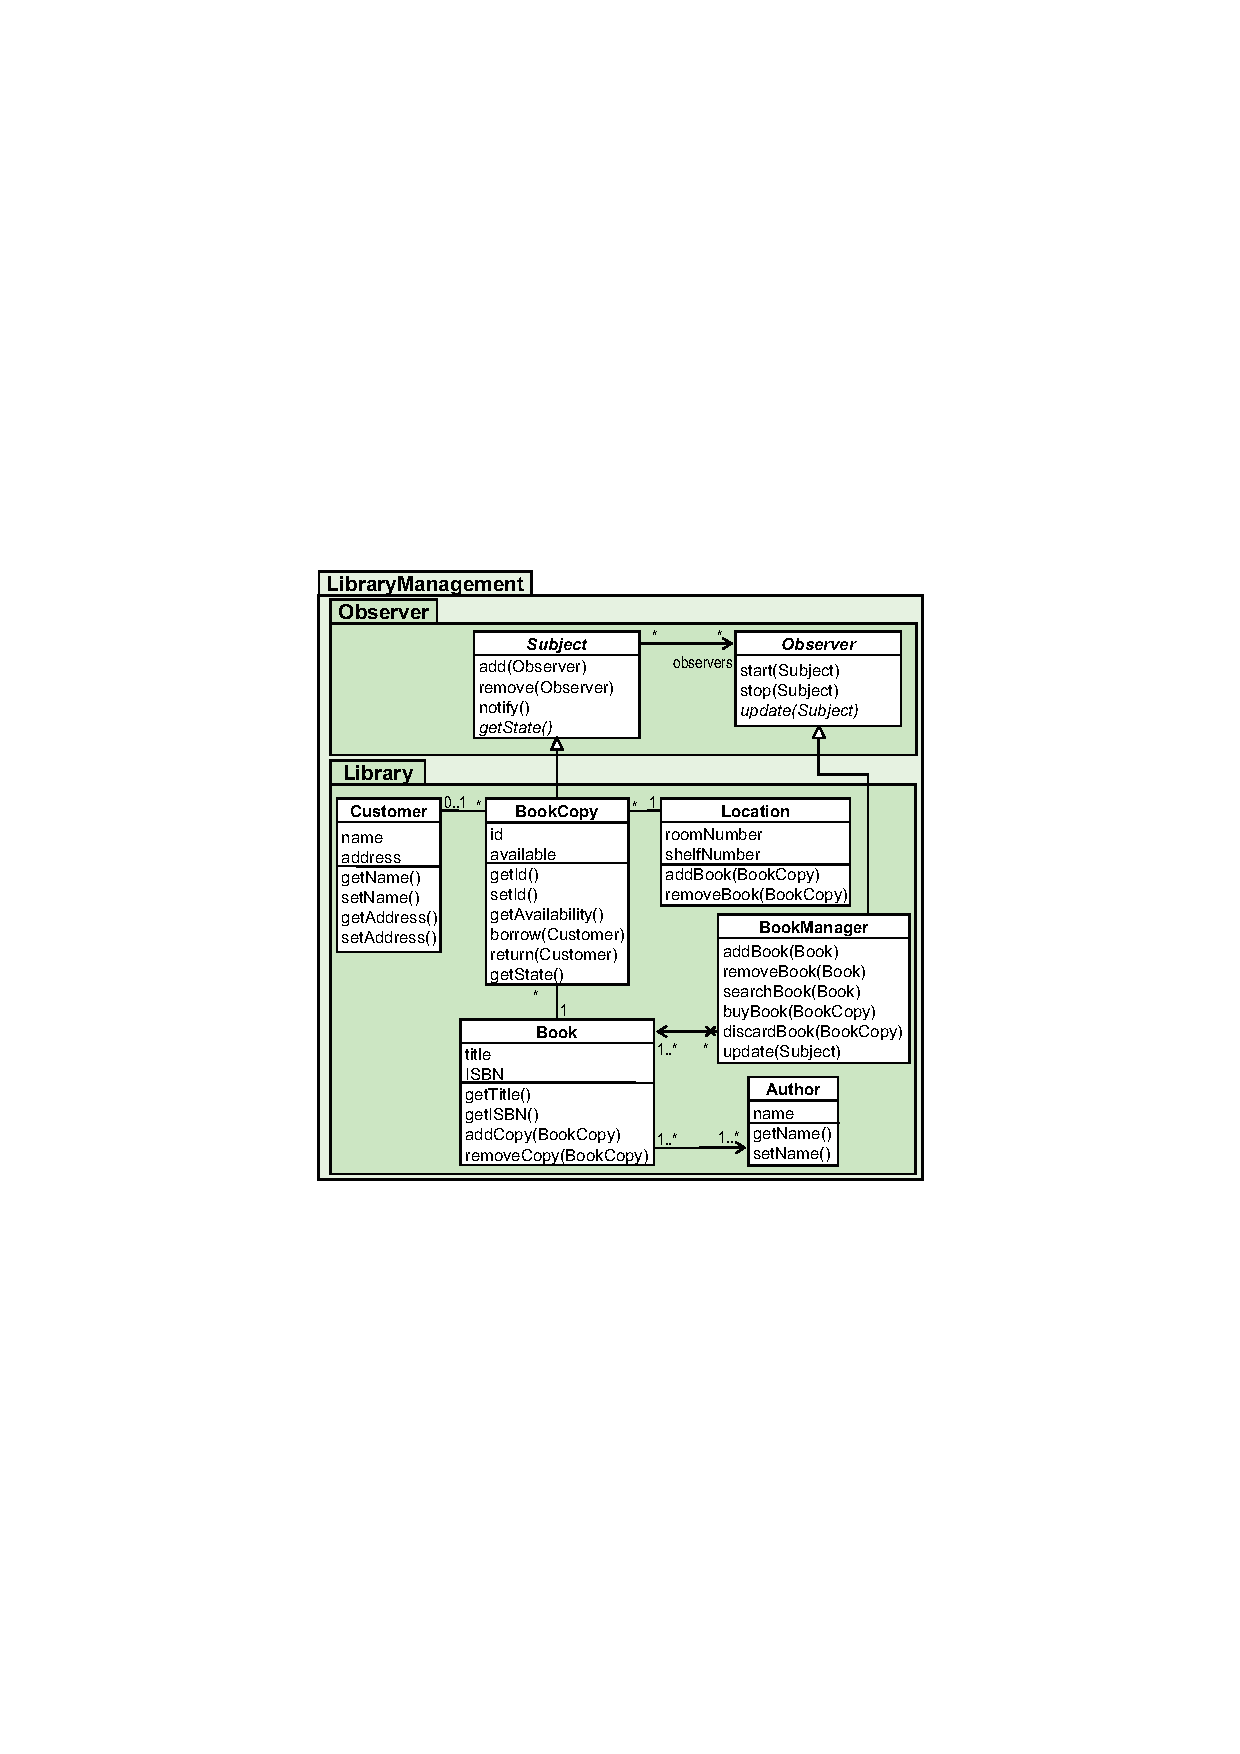
\includegraphics[width=0.4\linewidth]{figures/figure1}
	\caption{xxx (Quelle zitieren, wenn nicht selbst erstellt)}
	\label{fig:xxx}
\end{figure}

%-----------------------------------------------------------------------
\subsection{Tabellen}
%-----------------------------------------------------------------------

Jede Tabelle muss im Fließtext referenziertw werden. Für Tabellen gelten die selben Regeln, wie für Abbildungen (siehe dazu Abschnitt \ref{sec:abbildungen}).

Eine Beispiel einer Tabelle ist in Tabelle \ref{tab:xxx} zu finden:
\begin{table}
	\centering
	\begin{tabular}{| >{\bfseries}l | c | r | }
		\hline
			\rowcolor{orange} \bfseries Linksbündig & \bfseries Zentriert & \bfseries Rechtsbündig \\
		\hline
		\hline
			Zeile 1 & xxx & xxx \\\hline
			Zeile 2 & xxx & \dots \\\hline
			\multirow{2}{*}{Zeile3}
			& xxx & xxx \\\cline{2-3}
			& xxx & xxx \\\hline
		\hline
			\multicolumn{3}{| c |}{xxx} \\\hline
	\end{tabular}
	\caption{xxx (Quelle angeben)}
	\label{tab:xxx}
\end{table}

Bitte beachten Sie, dass Tabellen generell so einfach wie möglich gehalten werden sollen. Tabelle \ref{tab:xxx} dient unter anderem dazu Studierenden zu zeigen, wie Tabellen in \LaTeX\xspace erstellt werden können und wie Farben verwendet werden.